\documentclass[a4paper,kulak]{kulakarticle}

\usepackage{tikz}
\usetikzlibrary{positioning}
\usepackage[dutch]{babel}
\usepackage{hyperref}
\usepackage{graphicx}
\usepackage{amsmath, amssymb, amsthm}
\usepackage{siunitx}
\usepackage[toc,page]{appendix}
\renewcommand\appendixname{Bijlage}
\renewcommand\appendixpagename{Bijlagen}
\usepackage{pdfpages}


\title{Eindverslag}
\author{Groep 1: Safety First}
\address{
	Ruben Leenknecht, Emiel Vanspranghels, \\
	 Otto Meerschman, Staf Rys, Camille Louagie}
\date{vrijdag 21 mei, 2021}

\begin{document}

\maketitle
\tableofcontents

\newpage

\section{Inleiding}

\textbf{\large De groei en het verval van steden} \\
Meer en meer zien we een groei van het verstedelijkt gebied. Met deze groei nemen ook de problemen toe: zoals onder meer criminaliteit, lawaai en milieuvervuiling. Als we terugkijken in de tijd, zien we een meermaals voorkomende situatie. Steden zitten in een bloeiperiode, bereiken een verzadingspunt en kunnen daarna de vraag niet meer aan. Dit heeft een negatief effect op de economie en de efficiëntie in een stad. Zo was er ook de val van Rome, nadat deze een hoogtepunt had bereikt. Oude steden hadden dan wel een kleiner bereik, maar de relatie tussen technologie en stedelijke groei blijft dezelfde \cite{smartcities} . We staan opnieuw voor een keerpunt, waarbij we moeten kiezen tussen groeien of blijven steken.

We moeten de technologie die we voor handen hebben kunnen gebruiken om dit vastlopen te voorkomen. Met andere woorden moeten we van onze steden zogezegde  \lq slimme steden\rq\  maken \cite{taaladvies}. In ons dagdagelijkse leven worden we geconfronteerd met inefficiënte situaties die worden opgelost door een \lq slimme\rq\ aanpak. Daarom is het nodig mensen bewust te maken van het nut van deze slimme steden.\\ \\
\textbf{\large Slimme steden} \\
Maar wat zijn slimme steden nu juist? Met slim wordt de technologische innovatie bedoeld die opweegt tegen fysieke beperkingen. Een stad is een gebied van interacties en bijgevolg ook problemen en confrontaties \cite{sc}. In een kleine ruimte worden verscheidene dingen geconcentreerd samengebracht. Een stad heeft een veelheid aan functies en is pas doelmatig  wanneer ze deze functies met succes volbrengt \cite{synoniemen}. Een slimme stad wordt bereikt door stedelijke werking efficiënt te laten verlopen en door het vereenvoudigen van (openbare) diensten. Informatie- en communicatietechnologie (ICT), wordt gecombineerd met dagdagelijkse objecten om die interacties te verbeteren en stedelijke problemen te verminderen. Ondanks de vele vooruitgang van de afgelopen jaren, is het idee van een stad die volledig voorgeprogrammeerd gestuurd wordt, zonder menselijke tussenkomsten, voorlopig nog steeds een utopie. Nieuwe mogelijkheden en doorbraken zijn een drijfveer opdat dit ooit realiteit wordt \cite{proconsc}.\\ \\
\textbf{\large Zelfrijdende auto's} \\
Een van de middelen om de efficiëntie te verhogen in een stad is door het invoeren van zelfrijdende auto's die zelfstandig kunnen deelnemen aan het verkeer. Niet alleen wordt er extra tijd gecreëerd voor de bestuurder, die hij nuttiger kan spenderen, maar ook kunnen de auto's dichter op elkaar volgen en is het naleven van de verkeersregels verzekerd, mits de regels correct geïnterpreteerd worden. Dit kan ook voor een vermindering van het aantal verkeersongevallen zorgen en bijgevolg minder filedrukte. Het concept heeft niet alleen maar voordelen. Zo zouden hackers kunnen zorgen voor enorme verkeersproblemen. De verkeersgevallen die zich voordoen veroorzaken juridische conflicten in verband met aansprakelijkheid. Wie is verantwoordelijk wanneer iets misloopt? Is dit de bestuurder, de constructeur of de softwareontwikkelaar? Ook een inkomst van de overheid valt weg wanneer geen verkeersboetes of accijnzen op brandstof worden betaald. Daardoor zullen er meer belastingen op elektriciteit moeten geheven worden. Daarnaast zullen verschillende beroepen zoals buschauffeurs, rijinstructeurs en vrachtwagenchauffeurs overbodig worden, wat voor meer werkeloosheid onder minder geschoolden zal leiden \cite{procontracars}.

Ondanks de Vlaamse overheid autonoom rijden stimuleert met projecten zoals Smart Highway en project CONCORDA, staat men in Vlaanderen sceptisch tegenover het idee \cite{vbn}. Zo zou er een te grote psychologische drempel zijn \cite{scept}. Toch is er sprake van een grote marktpotentie. Bij de nieuwste auto's is er al sprake van een zeker mate van zelfstandigheid, zo kan men gealarmeerd worden bij het naderen van een andere bestuurder of een volle witte lijn. Bekende bedrijven zoals Google, Apple en Uber zijn volop bezig met de ontwikkeling van deze autonome wagens. Google werkt samen met verschillende autobouwers, waaronder Audi en Toyota en Apple heeft met hun project \lq Titan\rq\ al meer dan 50 autonome wagens op de openbare weg rijden \cite{bedrijven}. Er is geen ontkennen aan, zelfrijdende auto's hebben een toekomst. Om deze reden hebben wij besloten een miniatuurwagen te maken die in staat is om autonoom een voorgeprogrammeerde weg te volgen. Deze wagen laten we rijden in een miniatuur \lq smart city\rq\ samen met andere wagentjes met hetzelfde doel: het parcours met succes beëindigen. De taak is volbracht als het wagentje de verkeersregels volgt, het parcours juist interpreteert en geen botsingen veroorzaakt. We maken van de gekregen vrijheid gebruik om het wagentje volledig (in de mate van de gekregen vrijheid) naar onze hand te zetten.

\section{Klantenvereisten en ontwerpspecificaties}
Een zelfrijdende miniatuur robotwagen die zich rondbeweegt in een Slimme Stad zal aan bepaalde vereisten moeten voldoen en bepaalde dingen kunnen om zich zonder problemen te kunnen voortbewegen. Deze vereisten hangen vast aan hoe de Slimme Stad er uitziet en wat er van de gebruikers verwacht wordt


\subsection{Klantenvereisten}
De miniatuur miniatuurwagen moet zich volgens een voorgeprogrammeerde route door een modelstad kunnen voortbewegen waarbij de modelstad bestaat uit negen identieke kruispunten verbonden door straten van 1 meter lang ihij al dan niet mag door rijden of afslaan. Ook moet de miniatuurwagen een voorligger of obstakel kunnen detectern een grid. Hierbij volgt de miniatuurwagen een zwarte, volle volglijn. Bij de kruispunten is er een stopstreep en hangen er stoplichten op 75mm hoogte, die gemonteerd zijn op een tafelonderstel van 300 mm hoog. De miniatuurwagen moet stoppen bij de stopstreep en kunnen interpreteren wanneer en en op tijd kunnen stoppen om een botsing te vermijden indien nodig. Ook moet er een grafische gebruikersomgeving zijn waarmee relevante gegevens van de miniatuurwagen kunnen afgelezen worden en een manuele overname kunnen uitgevoerd worden via deze grafische gebruikersomgeving. De manuele overname moet in staat zijn een noodstop uit te voeren of de besturing van de miniatuurwagen over te nemen. De maximale kostprijs van de zelfrijdende miniatuur miniatuurwagen mag niet meer dan 3500 virtuele eenheden zijn.

\subsection{Ontwerpspecificaties}
De afmetingen van de miniatuurwagen worden beperkt tot 300 mm in de hoogte door de tafelonderstellen bij de kruispunten en 250 mm breedte door de breedte van de baan. De lengte van de miniatuurwagen valt vrij te kiezen, maar het moet wel haalbaar zijn om bijvoorbeeld bochten te nemen. De miniatuurwagen volgt een donkere volglijn op een lichte ondergrond van 25 mm breed. Aan een kruispunt interpreteert het wagentje een verkeerslicht dat zich bevindt op 75 mm boven de grond en knippert aan een frequentie van één Hertz. Het verkeerslicht is gemonteerd aan de voorkant van een tafelpoot waardoor het wagentje hem langs de rechterkant zal moeten detecteren.  Indien het verkeerslicht rood is, stopt de miniatuurwagen bij de stopstreep. Deze stopstreep is 50 mm dik en 25 cm lang. Het miniatuurwagentje kan ook voorliggers detecteren via een afstandssensor. Indien het een voorligger detecteert, vertraagt het wagentje of stopt het om zo een botsing te
vermijden. Het te volgen traject wordt een week op voorhand bekend gemaakt en kan
dan geprogrammeerd worden. De componenten van het prototype mogen verbonden worden via een experimenteerbord. De definitieve versie van de miniatuurwagen moet wel via een printplaat kunnen functioneren. Voor de microcontroller dient gebruik te worden
gemaakt van een NI myRIO of Raspberry Pi. Tussen de microcontroller en de motoren dient een motorshield te worden aangebracht, gezien dit een terugloopbeveiliging
bevat die beschadiging van de microcontroller voorkomt. Er moet ook een draadloze informatieoverdracht via LabVIEW aanwezig zijn die zich zal uiten op een zelfgemaakte grafische gebruikersomgeving. 


\section{Ontwerp}

\subsection{Chassis}
De ontwerpruimte werd sterk beperkt door de gelimiteerde materiaaldatabank. De belangrijkste keuzes betroffen de wielen, de motor, de microcontroller, het chassis, het type sensoren, de batterij en het experimenteerbord.
\\\\ \textbf{\large De wielen} \\
Voor de wielen van de miniatuurwagen hebben we gekozen voor de kleinste wielen met een diameter van 32 mm. Het voordeel aan deze wielen is dat ze meer nauwkeurigheid bieden bij het roteren van de miniatuurwagen en minder kracht nodig hebben om rond gedraaid te worden. Daarnaast kunnen kleinere wielen ook sneller ronddraaien, waardoor de elektrische motoren die de wielen aandrijven ook sneller ronddraaien. Dit leidt tot een verhoogde efficiëntie. Het nadeel aan deze wielen is echter wel dat de topsnelheid lager ligt. De wielen komen aan de voorkant, zoals te zien op figuur \ref{fig:Onderkant}, zodat dit het besturen van de miniatuurwagen vergemakkelijkt. De Bal Caster zullen we in het midden van achteren plaatsen. Deze zullen we proberen op dezelfde hoogte te plaatsen als de wielen door er plastic plaatjes onder te bevestigen. We positioneren de ball caster zodanig dat het chassis een minimale hoek maakt met de grond. Op deze manier verzekeren we dat de lijnsensor en de afstandssensor, respectievelijk, parallel en loodrecht staat met het grondoppervlak". De keuze voor deze wielen legt ook beperkingen op aan het type motoren.
\\\\ \textbf{\large De motor}

\begin{table}
	\centering
	\label{MotorenTab}
	\begin{tabular}{|l|r|r|r|}\hline
		Motor&	toeren/min &	km/h 	\\\hline
		100:1 HP&	310&	0.78\\\hline
		100:1&	130&	1.87 	\\\hline
		50:1 HP&	590&	2.71 \\\hline
		30:1&	1000&	3.56	\\\hline
		30:1 HP&	450&	6.03 	\\\hline
	\end{tabular}
	\caption{Berekening snelheid voor elke motor voor wielen met diameter 32 mm}

\end{table}
Wij kozen voor de 30:1 HP motor aangezien deze met een snelheid van ca. 6 km per uur het meest compatibel zijn met de gekozen wielen . Deze motor zorgt voor de hoogste topsnelheid met de wielen die we gekozen hadden. Om dit te bepalen hebben we enkele berekeningen uitgevoerd met het aantal toeren per minuut dat de motor maximaal kan draaien en de omtrek van de wielen \cite{converter}. Deze resultaten zijn te vinden in tabel \ref{MotorenTab}. Deze wielen en motoren zullen we plaatsen aan de voorkant van onze wagen. De motoren worden aan de onderkant van het chassis bevestigd om zo ons chassis hoger van de grond te krijgen en zo kan op die manier ook de lijnsensor aan de onderkant van het chassis geplaatst worden. Dit alles is te zien op figuur \ref{fig:Onderkant}.  

\begin{figure} [h]
	\begin{tikzpicture}
		\node [anchor=west] (Lijnsensor) at (-2,6) {\Large Lijnsensor};
		\node [anchor=west] (Wielen) at (-2,4) {\Large Wielen};
		\node [anchor=west] (Bal Caster) at (-2,1.5) {\Large Bal Caster};
		\begin{scope}[xshift=1.5cm]
			\node[anchor=south west,inner sep=0] (image) at (0,0) {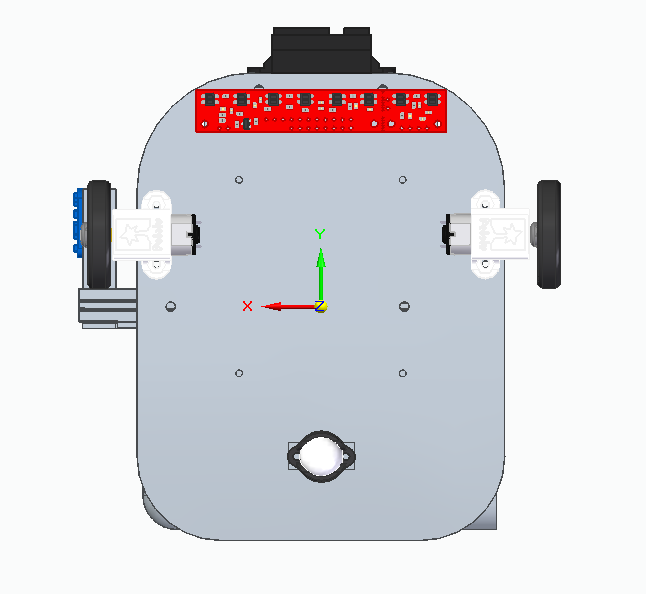
\includegraphics[width=.5\textwidth] {onderkant}
				
			};
			\begin{scope}[x={(image.south east)},y={(image.north west)}]
				%\draw[cyan,ultra thick,rounded corners] (0.4,0.55) rectangle (0.2,0.3);
				\draw [-stealth, line width=3pt, cyan] (Lijnsensor) -- ++(0.6,0.0);
				%\draw[cyan,ultra thick,rounded corners] (0.4,0.55) rectangle (0.2,0.3);
				\draw [-stealth, line width=3pt, cyan] (Wielen) -- ++(0.45,0.0);
				\draw [-stealth, line width=3pt, cyan] (Bal Caster) -- ++(0.75,0.0);
			\end{scope}
			
		\end{scope}
	\end{tikzpicture}
	\label{fig:Onderkant}
	\caption{Onderaanzicht van het CAD-model}
\end{figure}

\textbf{\large De microcontroller} \\
Een Raspberry Pi verbruikt zeer weinig stroom, wat een groot voordeel is wanneer je miniatuurwagentje op een batterij werkt. Daarnaast is het zeer makkelijk om informatie over de werking te vinden, aangezien deze microcontroller zoveel gebruikt wordt \cite{rasp}.
De Raspberry Pi wordt geplaatst op vier afstandsbussen van 15mm hoog waardoor hij op een platform komt te staan. Dit is te zien op figuur \ref{fig:afbchassis}. Op deze manier voorzien we voldoende ruimte voor de (plaatsing van de) sensoren, motoren, wielen en Maker Beams die nog op het chassis moeten komen. Op de Raspberry Pi komen twee kleine experimenteerborden die aan elkaar gelinkt zijn. Achter de Raspberry Pi ter hoogte van onze Bal Caster zullen we de powerbank op het chassis plaatsen. Deze past jammer genoeg juist niet onder de Raspberry waardoor hij niet onder het platform kan. De powerbank zorgt met zijn gewicht ervoor dat het massamiddelpunt van de wagen meer naar achteren en lager komt te liggen wat zorgt voor extra stabiliteit. De powerbank is ook makkelijk aan te sluiten op de Raspberry Pi en levert het juiste voltage voor de Raspberry Pi om te functioneren. 

\begin{figure} [h]
	\begin{tikzpicture}
		\node [anchor=west] (Batterij) at (-2,4) {\Large Batterij};
		\node [anchor=west] (Afstandssensor) at (-2,1) {\Large Afstandssensor};
		\node [anchor=west] (Microcontroller) at (-2,3) {\Large Microcontroller};
		\begin{scope}[xshift=1.5cm]
			\node[anchor=south west,inner sep=0] (image) at (0,0) {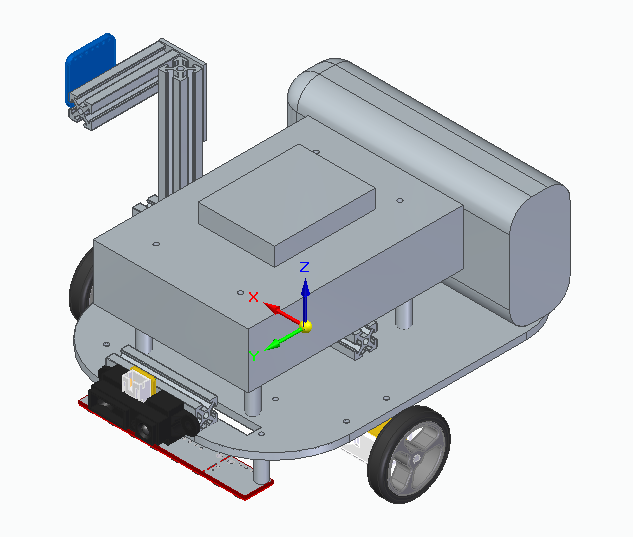
\includegraphics[width=0.5\textwidth]{afbchassis}
				
			};
			\begin{scope}[x={(image.south east)},y={(image.north west)}]
				%\draw[cyan,ultra thick,rounded corners] (0.4,0.55) rectangle (0.2,0.3);
				\draw [-stealth, line width=3pt, cyan] (Batterij) -- ++(01.1,0.0);
				%\draw[cyan,ultra thick,rounded corners] (0.4,0.55) rectangle (0.2,0.3);
				\draw [-stealth, line width=3pt, cyan] (Afstandssensor) -- ++(0.4,0.1);
				\draw [-stealth, line width=3pt, cyan] (Microcontroller) -- ++(0.4,0.0);
			\end{scope}
			
		\end{scope}
	\end{tikzpicture}
	\label{fig:afbchassis}
	\caption{De volledige miniatuurwagen}
\end{figure}

Het chassis is handmatig ontworpen naar de behoeften van het miniatuurwagentje en zal ge-3D-print worden. Dit chassis zal 140 mm lang, 110 mm breed en 3 mm dik zijn met afgeronde hoeken, zoals te zien op figuur \ref{fig:chassis}. Hiermee bekomen we een chassis waarmee we genoeg ruimte hebben in de lengte om onze microcontroller en onze powerbank op te plaatsen. De afgeronde hoeken zorgen ervoor dat bochten makkelijker genomen kunnen worden. Vooraan het chassis zal er een gleuf voorzien worden van 6,5 mm breed en 45,8 mm lang voor de verbindingsdraden naar de lijnsensor die onder het chassis hangt, zie figuur \ref{fig:Onderkant}. Er zullen ook gaten in het chassis bevinden die kunnen gebruikt worden voor het bevestigen van componenten met schroeven en moeren. Het chassis zal aan een dichtheid van 70\% ge-3D-print worden zodat hij genoeg steun kan bieden en niet zal doorzakken.
\begin{figure}[h]
	\centering
	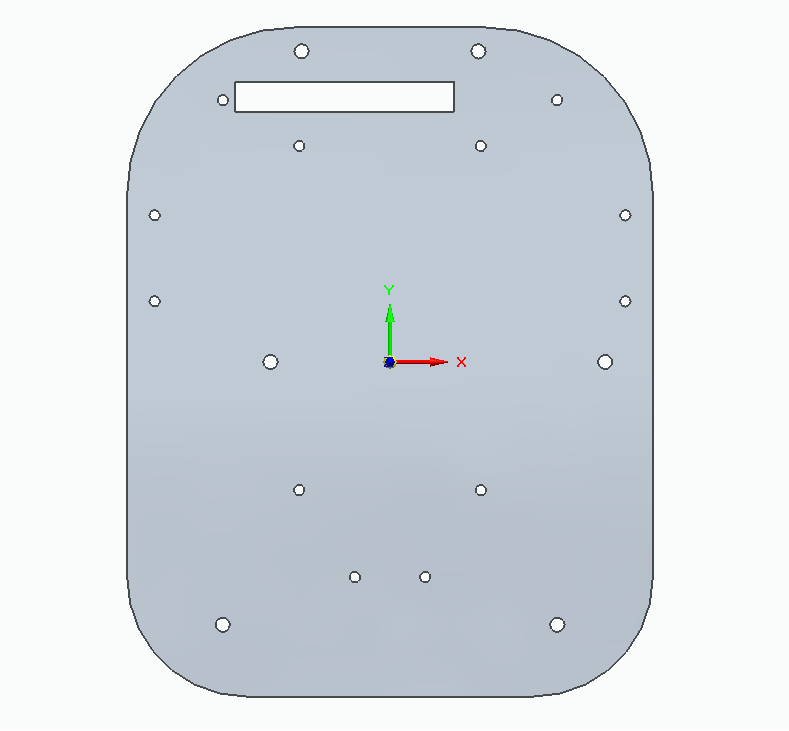
\includegraphics[width=.5\textwidth] {chassis3d}
	\caption{CAD-model van het zelf ontworpen chassis.}
	\label{fig:chassis}
\end{figure}

\subsection{Sensoren}
De kleurensensor zal bevestigt worden aan een MakerBeam-staaf op een hoogte van 75mm van de grond zodat deze het verkeerslicht, die op dezelfde hoogte hangt, kan detecteren. Hierbij zal een constructie van MakerBeams ervoor zorgen dat de kleurensensor kan verplaatst worden in alle richtingen indien nodig. \ref{fig:Linksaanzicht} Deze constructie bestaat uit een MakerBeam die horizontaal in het midden van ons chassis ligt onder de Raspberry Pi met daarop een MakerBeam verticaal omhoog aan het rechter uiteinde. De kleurensensor wordt bevestigd aan de horizontale MakerBeam

\begin{figure}[h]
	\begin{tikzpicture}
		\node [anchor=west] (Afstandsbussen) at (-2,2) {\Large Afstandsbussen};
		\node [anchor=west] (Kleurensensor) at (-2,5) {\Large Kleurensensor};
		\begin{scope}[xshift=1.5cm]
			\node[anchor=south west,inner sep=0] (image) at (0,0) {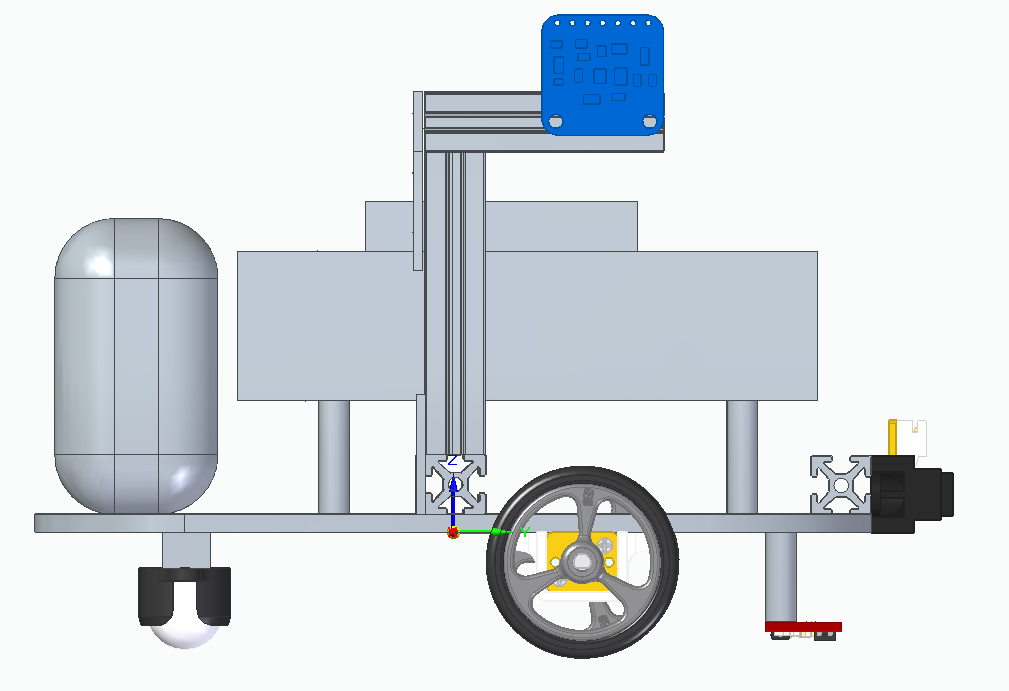
\includegraphics[width=.5\textwidth] {rechterkant}
				
			};
			\begin{scope}[x={(image.south east)},y={(image.north west)}]
				%\draw[cyan,ultra thick,rounded corners] (0.4,0.55) rectangle (0.2,0.3);
				\draw [-stealth, line width=3pt, cyan] (Afstandsbussen) -- ++(0.55,0.0);
				\draw [-stealth, line width=3pt, cyan] (Kleurensensor) -- ++(0.75,0.0);
			\end{scope}
			
		\end{scope}
	\end{tikzpicture}
	\label{fig:Linksaanzicht}
	\caption{Linkeraanzicht van de miniatuurwagen met de constructie voor de kleurensensor}
\end{figure}

Voor de afstandssensor hebben we gekozen voor een analoge sensor, opdat we nauwkeurig kunnen meten hoever het wagentje verwijderd is van een obstakel of een andere weggebruiker. Doordat we dit onderscheid kunnen maken moet onze miniatuur miniatuurwagen niet direct stoppen wanneer hij een voorligger detecteert, maar kan hij er voor  zorgen dat hij eerst wat trager rijdt vooraleer volledig te stoppen. Deze afstandssensor plaatsen we logischer wijze aan de voorkant van ons chassis aan een MakerBeam zodat hij zo vroeg mogelijk een voorligger kan detecteren aangezien zijn detectie bereik maar 100mm is. 

De lijnsensor wordt gebruikt om de volglijn te detecteren. Hierbij hebben we een digitale sensor gekozen omdat deze compatibel is met de Raspberry Pi microcontroller en de sensor geen onderscheid moet kunnen maken tussen de soort lijn. Deze wordt aan de voorkant onder het chassis bevestigd met behulp van afstandsbuizen zodat deze de volglijn als eerst detecteert en we zo sneller correcties kunnen uitvoeren. Aangezien de sensor dicht bij de wielen ligt zal het wagentje ook nauwkeuriger bewegen.

Het volledige ontwerp is te zien in figuur \ref{fig:chassis}.


	
\section{Evaluatie}

\subsection{Planning}
Tot en met week 5 is alles verlopen zoals gepland en vastgelegd in de Gantt-grafiek. De documenten met betrekking tot de planning zijn afgewerkt net zoals het ontwerp van de chassis en het CAD-model. Het bestellen van de onderdelen vond later plaats dan verwacht, vanwege de plaatsing bij de bieding. Dit heeft ons met een achterstand doen starten aan het programmeren en assembleren. Het team was van plan om te beginnen met de assemblage in week 6, echter wordt dit een week uitgesteld vanwege een probleem met de microcontroller. Het programmeren van de sensoren verliep vlot, enkel het programmeren in verband met de aansturing van het wagentje zal iets meer tijd innemen dan ingerekend. Dit wordt dan wel gecompenseerd met het maken van het CAD-model dat minder tijd innam dan voorspeld, waardoor we nog altijd op schema zitten. Ook het schrijven van het verslag verloopt volgens schema. De tijd voorzien tijdens de lessen wordt efficiënt gebruikt, waardoor het werk buiten de lessen wordt beperkt tot een minimum.


\subsection{Financiën}

Doordat we de laatste keuze hadden bij het bestellen, liepen we achter op onze planning, onze financiële situatie kende hier dan weer voordelen door. We zijn gestart met een budget van 3500 kredietpunten, dat werd gereduceerd tot een tegoed van 1768 na het plaatsen van een eerste bestelling. In deze  order werden alle grote onderdelen en zaken die we zeker nodig hadden besteld.  Aan onze eerste levering ontbraken nog Maker Beams en afstandsbussen. Onze tweede bestelling zal voorlopig 61 kredietpunten kosten, waardoor we stranden op een budget van 1646 kredietpunten. Door eigen keuze wordt het chassis zelf ontworpen en 3D-geprint. Dit is vermoedelijk een grote kost die werd geschat op 500 kredietpunten. Onze financiële toestand zorgt ervoor dat we in een comfortabele situatie zitten en kunnen we het ons veroorloven om fouten te maken en risico's te nemen. 


\section{Besluit}


Met het gegeven budget hebben we de mogelijkheid een correct functionerend wagentje te bouwen die in staat is autonoom een voorgeprogrammeerd pad te volgen zonder hinder te veroorzaken of de verkeersregels te overtreden. Dit project toont op kleine schaal aan dat een smart city en meer specifiek, zelfrijdende wagens minder utopie en meer werkelijkheid worden.
Zelfrijdende wagens kennen zeker een toekomst en hebben hun nut al meermaals bewezen. De weg naar een wereld met autonome wagens is lang, maar wordt stilaan meer en meer bereden.



	\bibliographystyle{plain} %De stijl van de bibliografie
	\bibliography{bibliografietv} %De bibliografie zelf
\begin{appendices}
	\section*{Planningsdocumenten} %De goede titel
	\renewcommand\refname{} %De oude titel verwijderen
	\vspace{-2\bigskipamount} %De cursor terugzetten
	
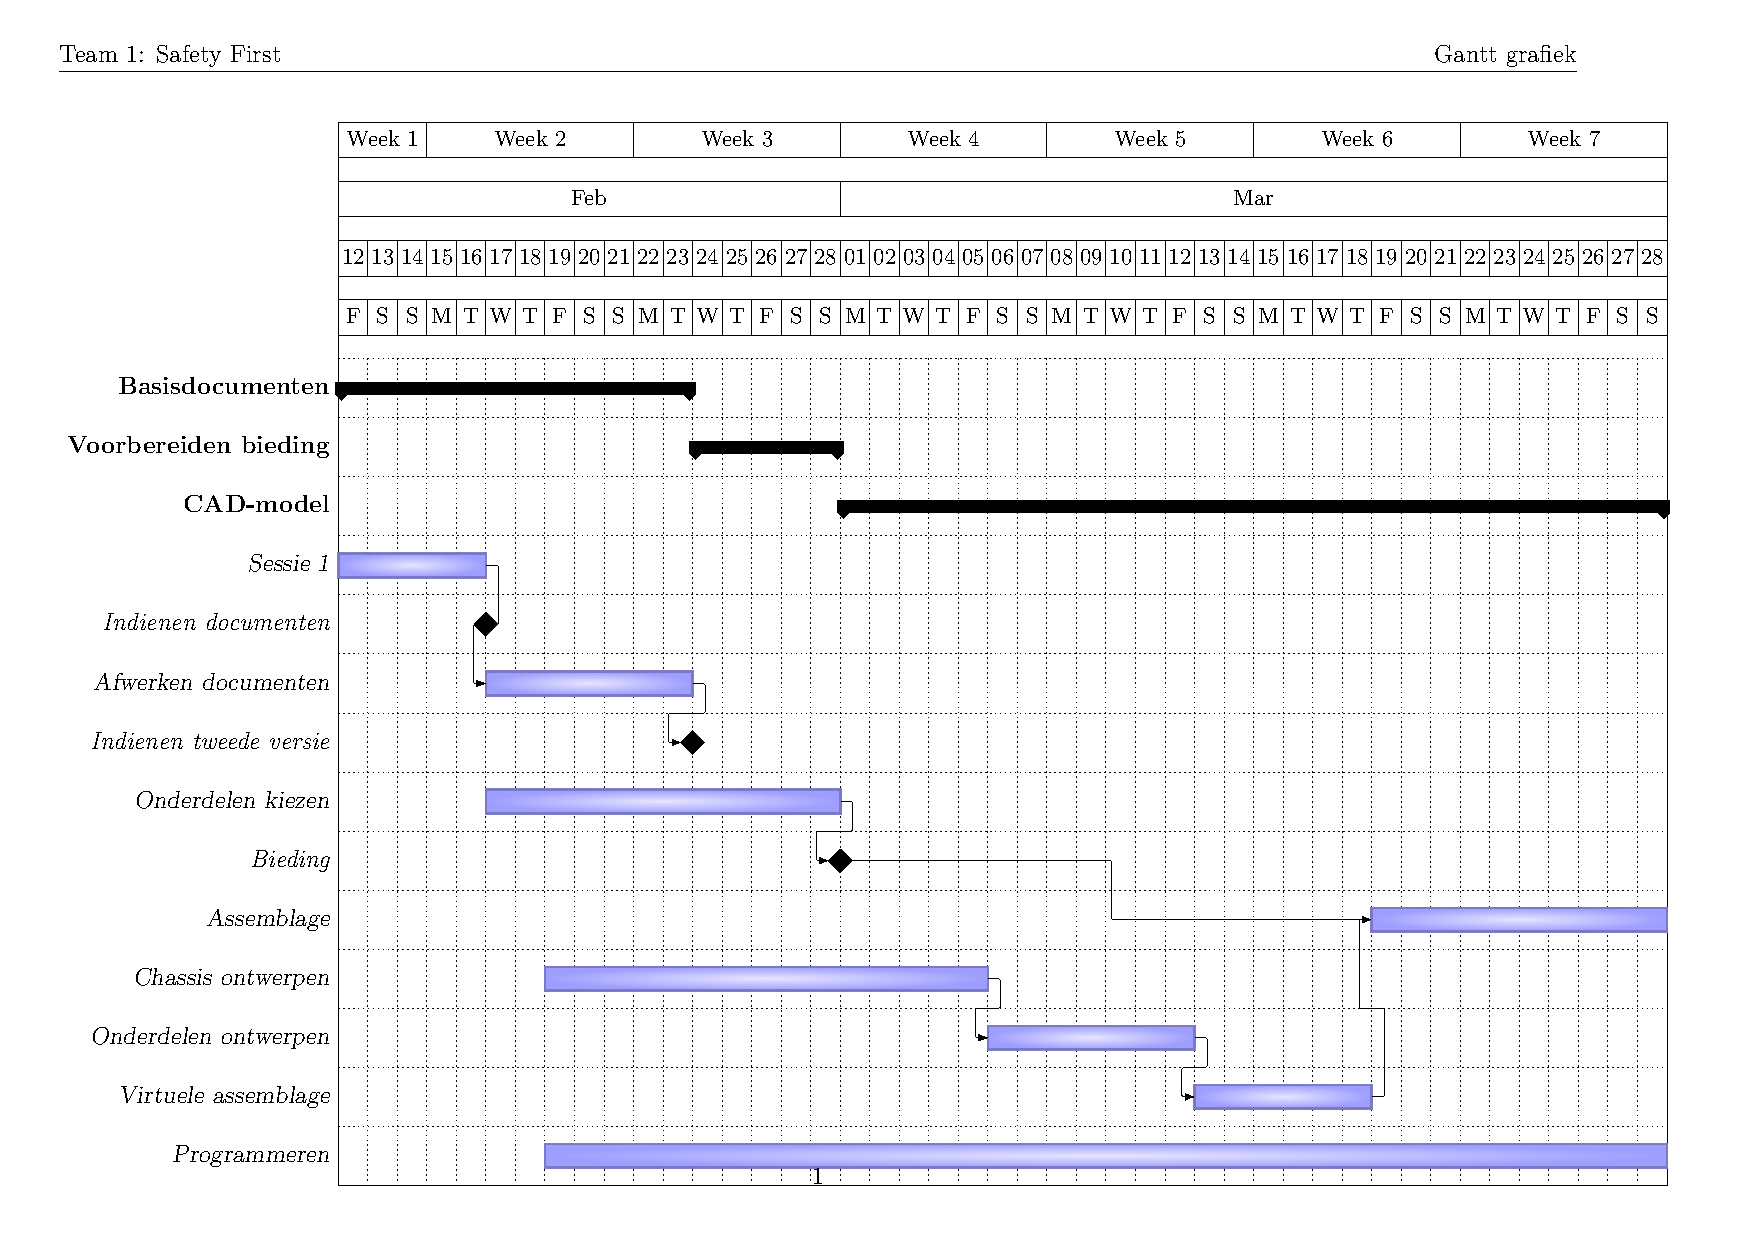
\includepdf[pages=-]{ganttchart.pdf}

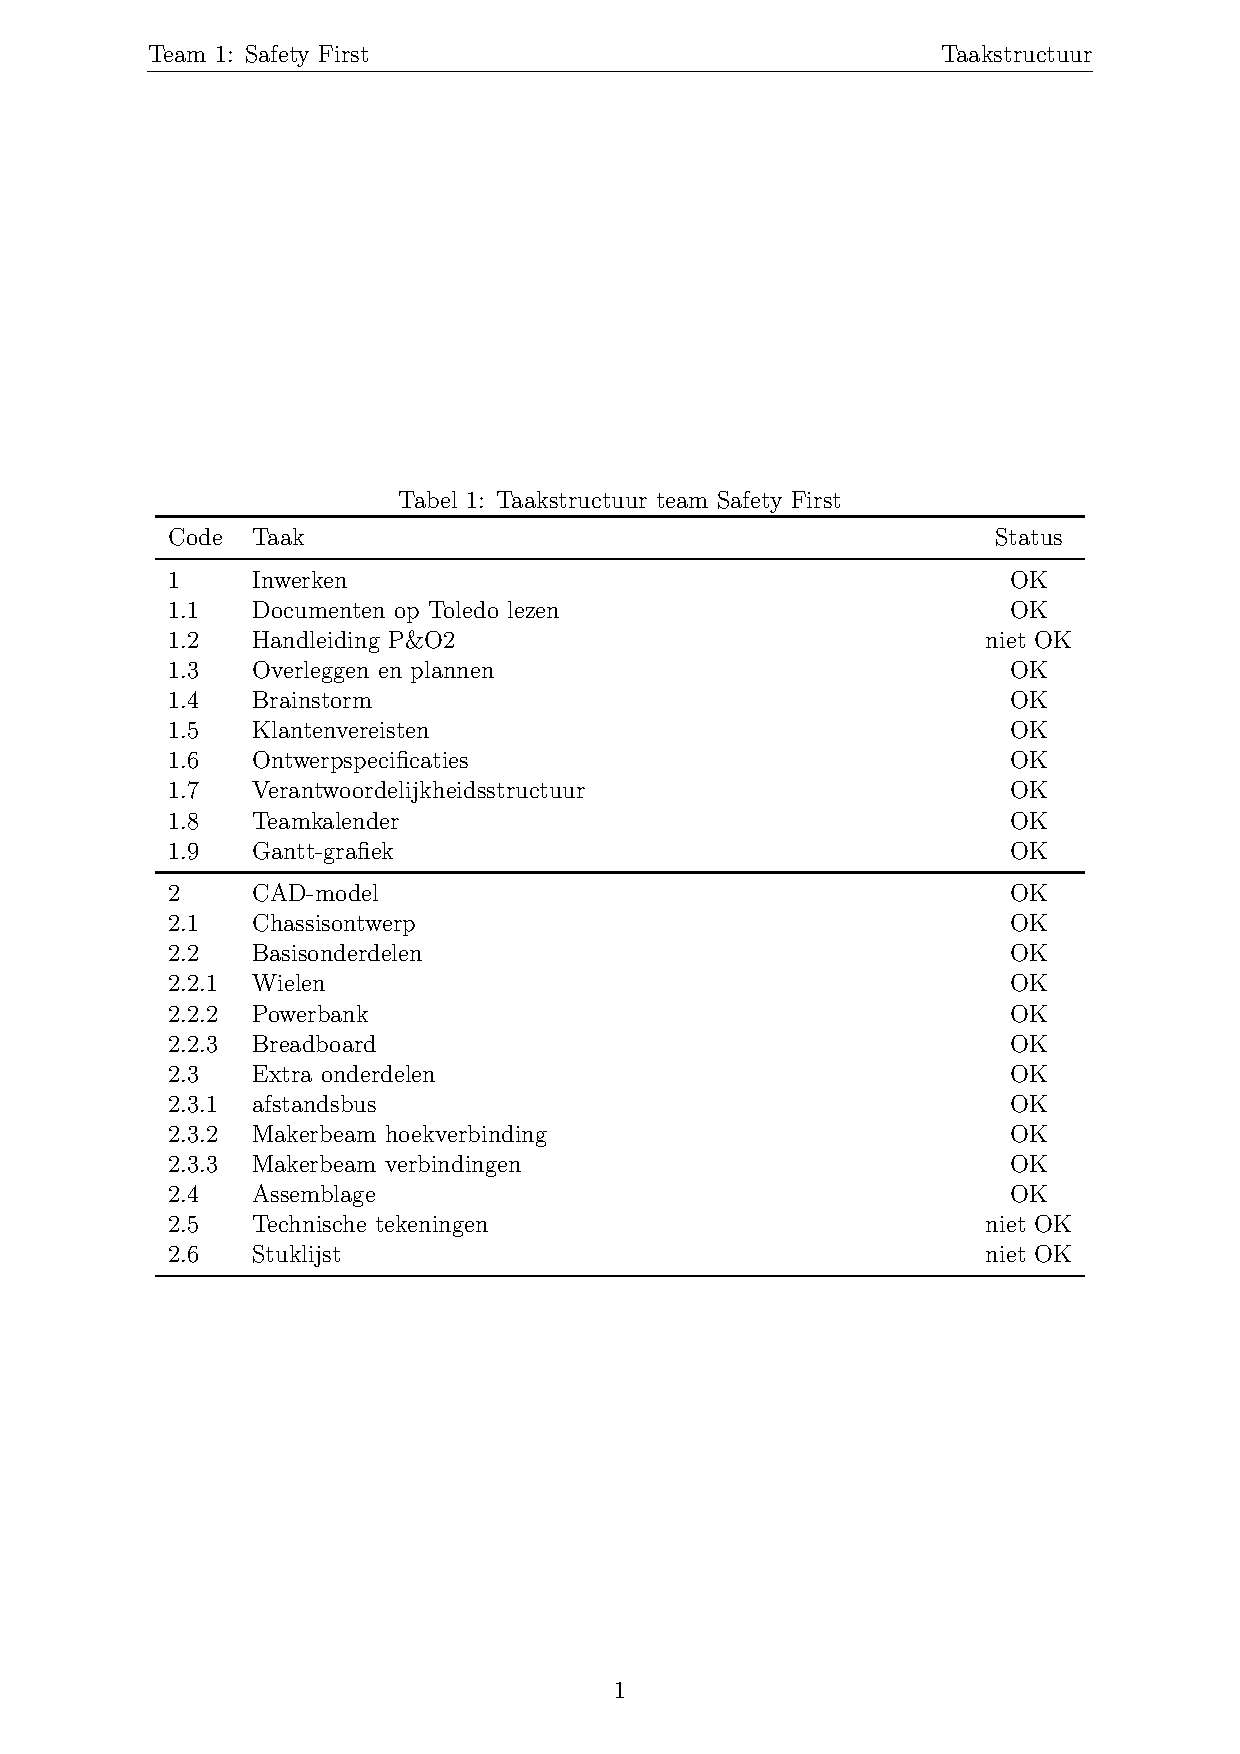
\includepdf[pages=-]{taakstructuur.pdf}

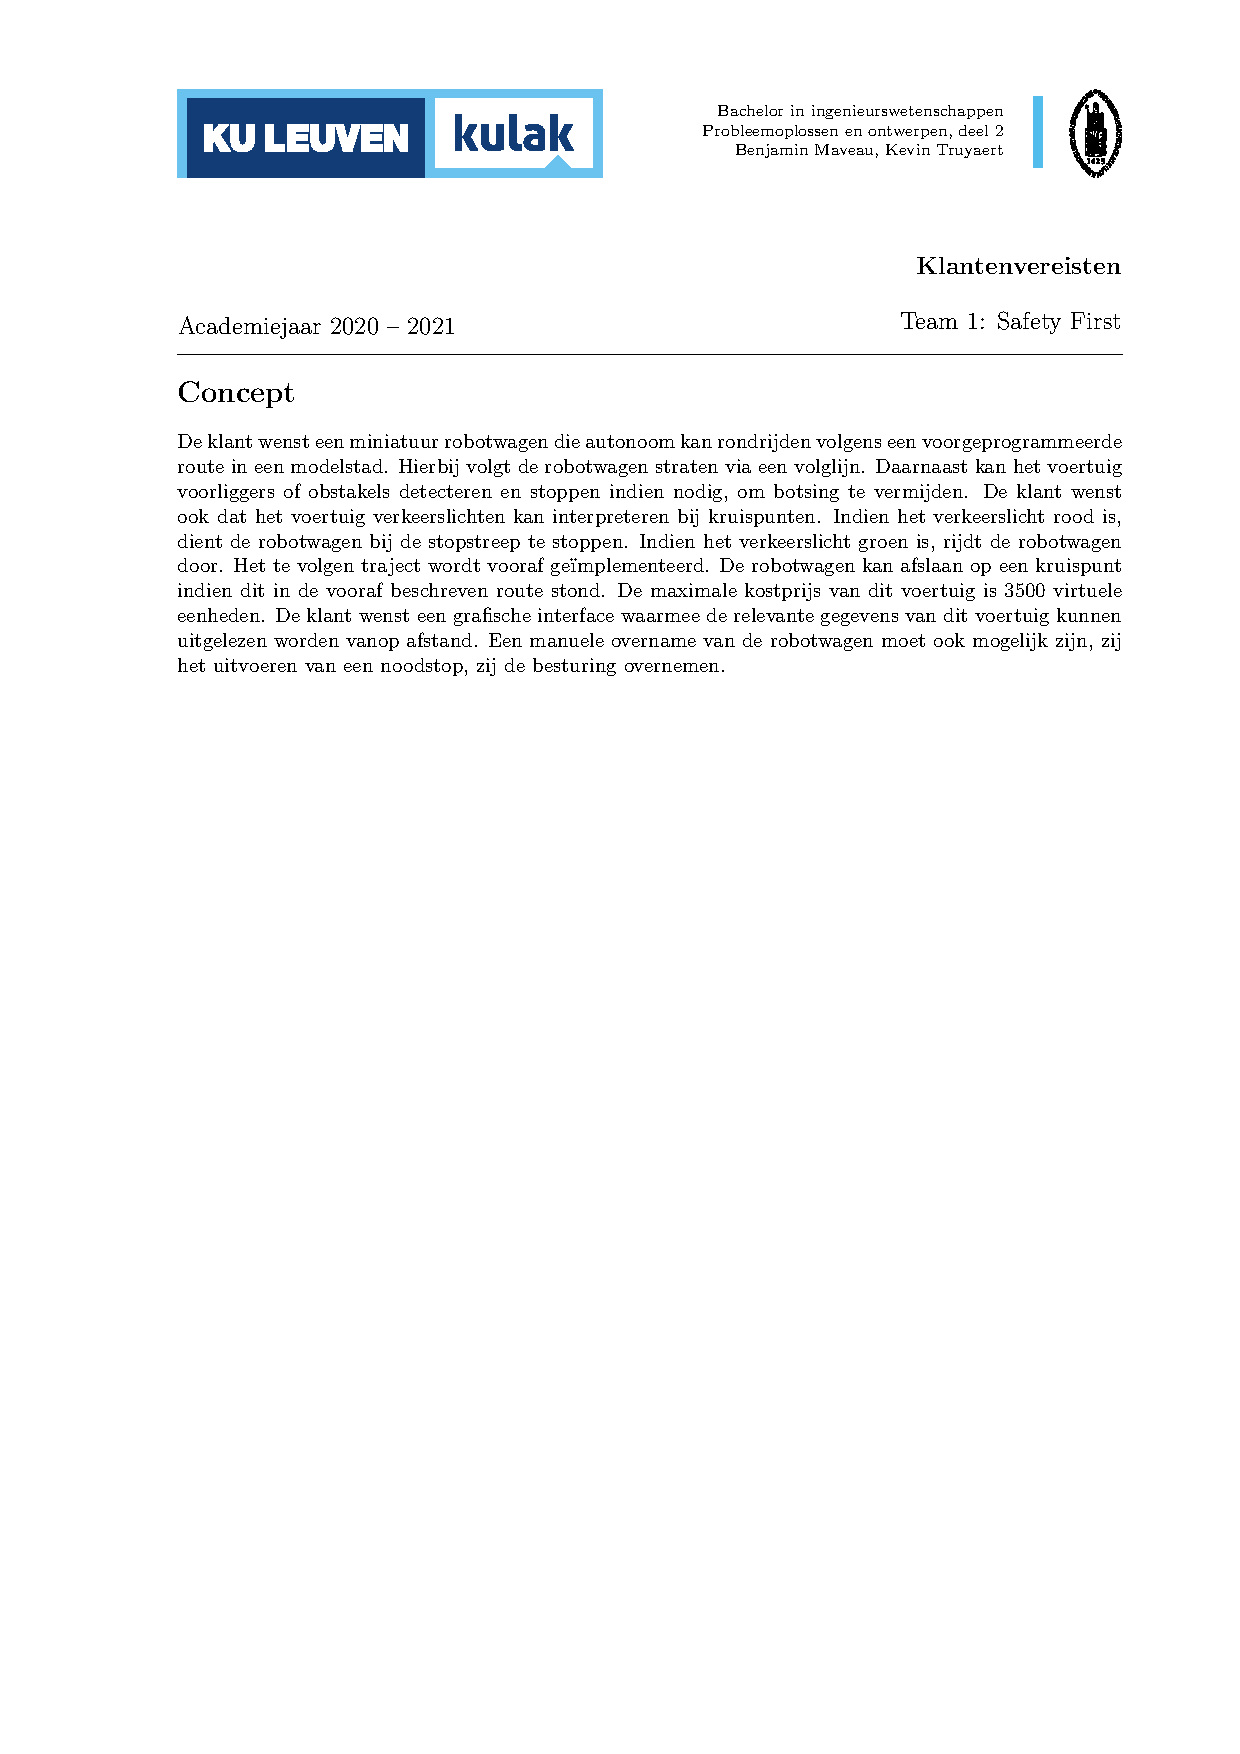
\includepdf[pages=-]{klantenvereisten.pdf}
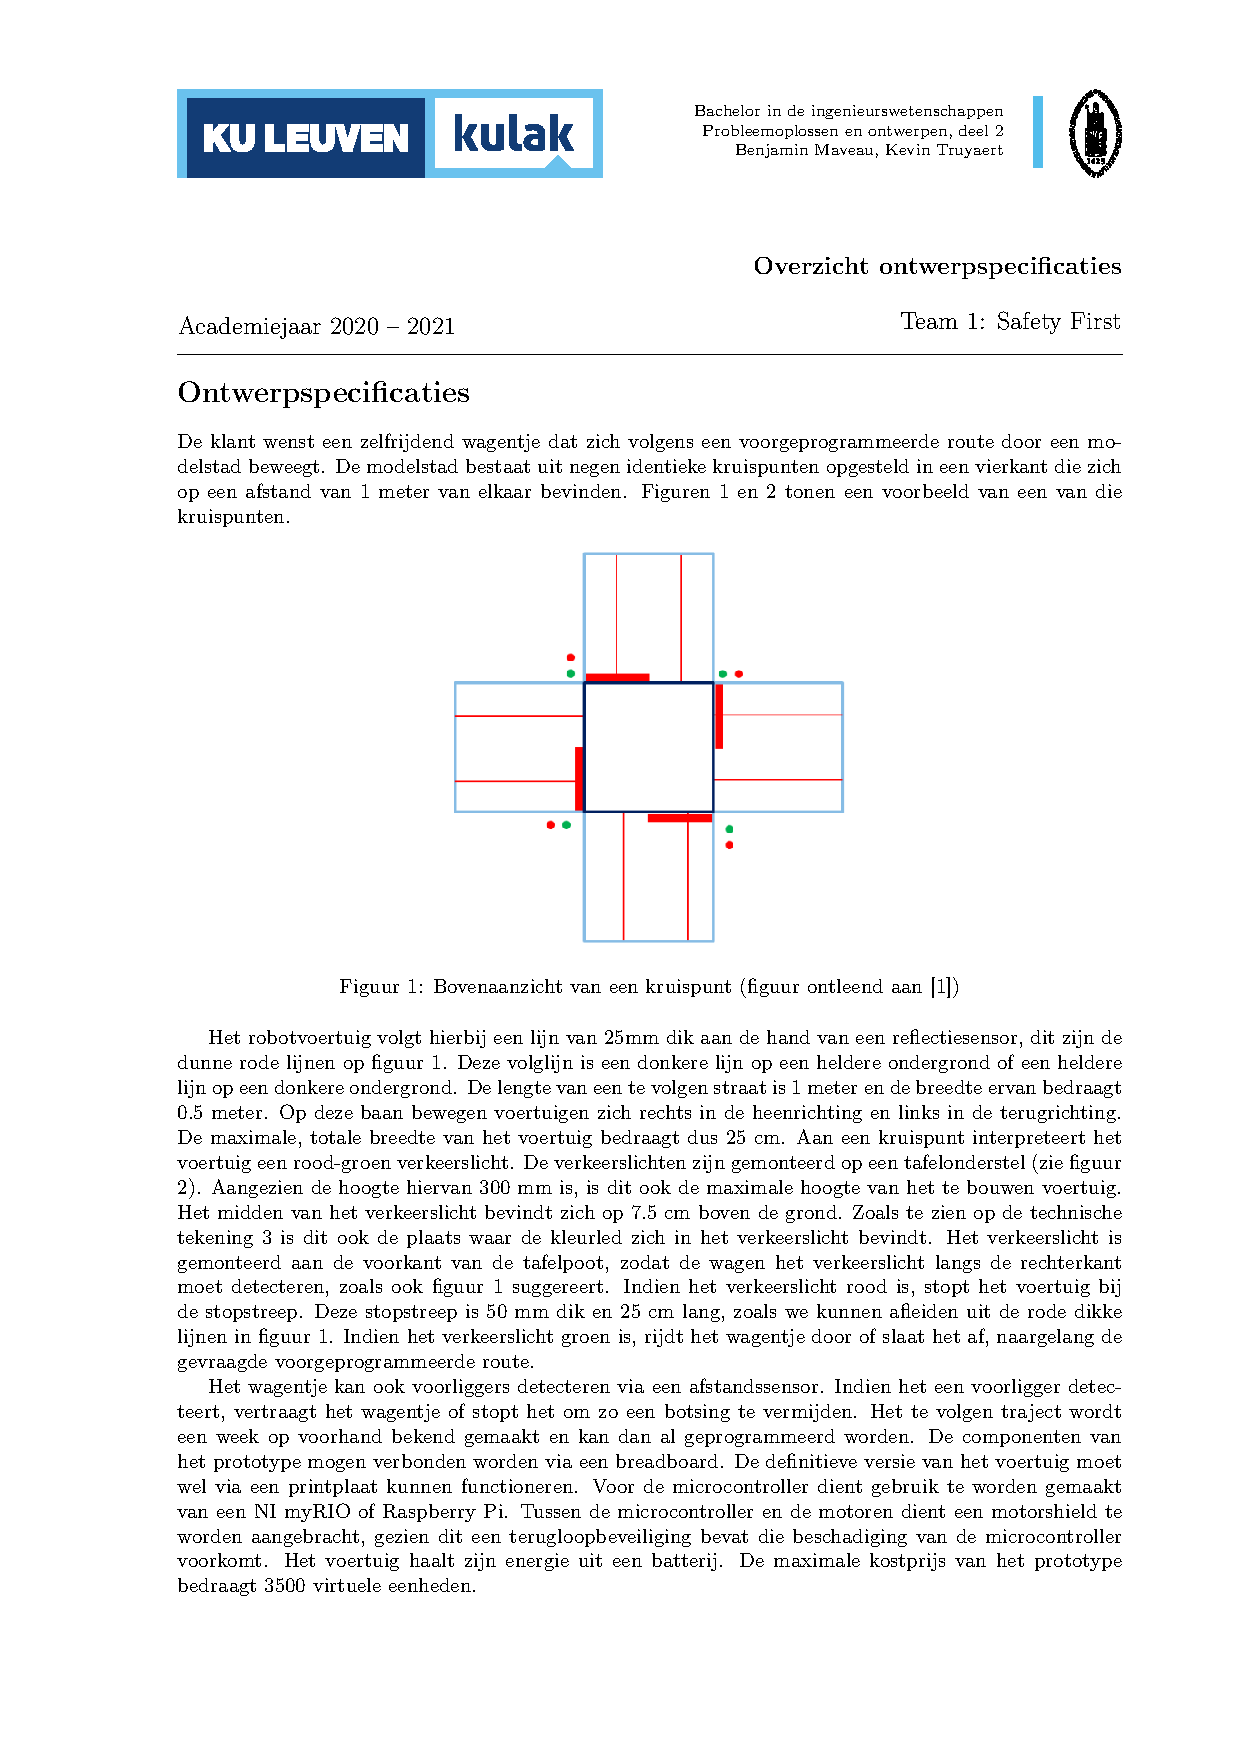
\includepdf[pages=-]{ontwerpspecificaties.pdf}

\end{appendices}




\end{document}